\documentclass[conference]{IEEEtran}
\IEEEoverridecommandlockouts
% The preceding line is only needed to identify funding in the first footnote. If that is unneeded, please comment it out.
\usepackage{cite}
\usepackage{amsmath,amssymb,amsfonts}
\usepackage{algorithmic}
\usepackage{graphicx}
\usepackage{textcomp}
\usepackage{xcolor}
\def\BibTeX{{\rm B\kern-.05em{\sc i\kern-.025em b}\kern-.08em
    T\kern-.1667em\lower.7ex\hbox{E}\kern-.125emX}}
\begin{document}

\title{Projektbericht: Spotify Analyse\\}

\author{\IEEEauthorblockN{1\textsuperscript{st} Eric Kaufmann}
\IEEEauthorblockA{
Jena, Germany \\
eric.kaufmann@uni-jena.de}
\and
\IEEEauthorblockN{2\textsuperscript{nd} Maria Gogolev}
\IEEEauthorblockA{
Jena, Germany \\
maria.gogolev@uni-jena.de}
}

\maketitle

\begin{abstract}
In diesem Projektbericht wurden zwei Datensätze von Kaggle verwendet, verbunden und anschließend analysiert. Dabei werden Merkmale von Songs durch die Einteilung in Playlisten betrachtet. Mittels Erstellung einer neuen Metrik können Eigenschaften populärer Songs bestimmt und Veränderungen im Laufe der Zeit verglichen werden.
\end{abstract}

% \begin{IEEEkeywords}
% component, formatting, style, styling, insert
% \end{IEEEkeywords}

\section{Datensätze}

Als Datensätze wurden zwei von kaggle.com verwendet:
\begin{enumerate}
    \item Spotify 1.2M+ Songs\footnote{siehe https://www.kaggle.com/datasets/rodolfofigueroa/spotify-12m-songs}
    \item Spotify Playlists\footnote{siehe https://www.kaggle.com/datasets/andrewmvd/spotify-playlists}
\end{enumerate}
Ersteres besteht, wie der Name es schon verdeutlicht, aus ca. 1.2 Millionen (1,204,025 genau) unterschiedlichen Spotify Songs. Zu jedem Song sind dabei 24 Eigenschaften gegeben. Eine Auflistung aller Eigenschaften mit Beschreibung ist in Tabelle \eqref{tab:song_feat} zu finden. Der Datensatz liegt als CSV vor umfasst ungefähr 346MB. Die Daten wurden dabei mittels der offiziellen Spotify-API generiert. Jeder Song kann mittels einer eindeutigen ID beschrieben werden. Durch eine GET-Anfrage auf \textit{https://api.spotify.com/v1/tracks/\{id\}} können Informationen zum Album, Songtitel, Artisten und Publikationsdatum extrahiert werden. Mittels zweiter GET-Anfrage auf \textit{https://api.spotify.com/v1/audio-features/\{id\}} können die restlichen Eigenschaften, wie \textit{danceability}, \textit{energy} oder \textit{liveness} bestimmt werden.

\begin{table}[h]
    \caption{Beschreibung der Spalten des Spotify 1.2M+ Songs Datensatz}
    \begin{center}  
    \begin{tabular}{ll}
        Eigenschaft & Beschreibung \\ \hline
        id & Song-ID \\
        name & Songtitel \\
        album & Albumtitel \\
        album\_id &  Album-ID\\
        artists & Liste der Artisten \\
        artists\_ids & Liste der Artisten-IDs \\
        track\_number & Tracknummer des Songs im Album \\
        disc\_number & Albumnummer \\
        explicit & Song ist explicit\\
        danceability & Eignung des Songs zum tanzen ($\in [0,1]$) \\
        energy & Intensität und Aktivität des Songs ($\in [0,1]$) \\
        key & Tonart \\
        loudness & Lautstärke (dB) \\
        mode & Modus (Dur/Moll) \\
        speechiness & Sprachanteil ($\in [0,1]$) \\
        acousticness & Akustik eines Songs ($\in [0,1]$) \\
        instrumentalness & Instrumentalanteil ($\in [0,1]$) \\
        liveness & Wahrscheinlichkeit einer Liveübertragung ($\in [0,1]$) \\
        valence & Wertigkeit ($\in [0,1]$, 0=negativ und 1=positiv) \\
        tempo & Tempo (BPM) \\
        duration\_ms & Dauer (ms) \\
        time\_signature & Taktart \\
        year & Veröffentlichungsjahr \\
        release\_date & Veröffentlichungsdatum (YYYY-MM-DD)
    \end{tabular}
    \end{center}
    \label{tab:song_feat}
\end{table}

Der Datensatz ermöglicht es Songs anhand von Eigenschaften zu sortieren. Beispielsweise kann man verschiedene Eigenschaften wie die \textit{danceability}, \textit{valence} oder \textit{energy} der Songs über die Zeit betrachten. Eine andere exemplarische Anwendungsmöglichkeit ist ein Algorithmus zur Songempfehlung, bei dem man Songs mit ähnlichen Eigenschaften versucht zu verbinden. 

Um die Songs besser unterteilen zu können wurde in dieser Analyse ein zweiter Datensatz verwendet, der Spotify Playlist Datensatz. Dieser besteht aus ca. 2.8 Millionen unterschiedlichen Songs, die in ca. 162 Tausend Playlists von ungefähr 16 Tausend User eingeteilt sind. Trotz einer Größe von ca. 1.8 GB ist der Aufbau des Datensatzes recht einfach. Wie in Tabelle \eqref{tab:feat_playlist} erkennbar besitzt der Datensatz nur vier Spalten. Dabei hat ein User mit einer \textit{user\_id} eine Playlist mit der Playlistbezeichnung \textit{playlistname} angelegt. Songs, bestimmt durch den \textit{trackname} und \textit{artistname}, können somit einer Playlist zugehörig sein. Selbstverständlich können dabei Songs mehrfach vorkommen, wenn sie beispielsweise in unterschiedlichen Playlists enthalten sind oder in einer Playlist sogar mehrfach aufkommen.

\begin{table}[h]
    \caption{Beschreibung der Spalten des Spotify Playlist Datensatz}
    \begin{center}  
    \begin{tabular}{ll}
        Eigenschaft & Beschreibung \\ \hline
        user\_id & User-ID eines Spotify Nutzers \\
        artistname & Name des Artisten \\
        trackname & Songtitel \\
        playlistname & Playlistbezeichnung
    \end{tabular}
    \end{center}
    \label{tab:feat_playlist}
\end{table}

Mögliche Anwendungsfelder dieser Playlist ist beispielsweise die Untersuchung der Popularität einiger Songs durch die Anzahl der Aufkommen des Liedes in unterschiedlichen Playlisten. Mehr dazu später. 

Um die Songeigenschaften des ersten Datensatzes mit den Playlisteinteilungen des zweiten Datensatzes zu verbinden, müssen die beiden Datensätze verbunden werden. Dafür versuchen wir an den Playlist-Datensatz mittels left-join die Eigenschaften anzuheften. Dabei sollen die gemeinsamen Schlüssel der Songtitel mit Artisten sein. Um dies zu erreichen müssen jedoch vorher die Daten vorbereitet werden. Dafür wurden zunächst die Spaltennamen \textit{name} und \textit{artists}, beim Spotify 1.2M+ Datensatz, bzw. \textit{trackname} und \textit{artistname}, beim Spotify Playlistdatensatz, vereinfacht und in \textit{track} und \textit{artist} umbenannt. Somit sind die beiden Schlüssel gleich bezeichnet. 

Der nächste Schritt ist es die Liste von Artisten, welche in jeder Zeile der \textit{artist}-Spalte beim Spotify 1.2M+ Songs Datensatz zu finden ist, aufzusplitten. Diese haben nämlich eine folgende Form:

$$
    [\text'\text{artist}_1\text', \text'\text{artist}_2\text', \dots, \text'\text{artist}_n\text'].
$$

Ziel ist es, dass die Zeile des Datensatzes $n$-Mal repliziert wird und in jeder neuen Zeile nur der jeweilige $\text{artist}_i$ steht. Zum Schluss wurden die Datentypen aller Spalten angepasst und unrealistische Werte (z.B. Veröffentlichungsjahr 0) aussortiert. 

Nach dieser Vorbereitung der Daten ist es nun möglich den left-join des Spotify 1.2M+ Songs Datensatz an den Spotify Playlist Datensatz über die gemeinsame Schlüssel \textit{track} und \textit{artist} durchzuführen. Zur Vereinfachung der späteren Analyse wurde anschließend alle Zeilen mit \textit{NA}-Werten aus dem verbundenen Datensatz entfert. Somit werden auch alle Zeilen entfert, bei dem der Spotify Playlist Datensatz keine Werte für Songs aus dem Spotify 1.2M+ Songs Datensatz findet.

Die Verbindung der Datensätze hat jedoch einen großen Datenverlust zur Folge. Nach der Vorverarbeitung der einzelnen Datensätze sind beim Spotify 1.2M+ Songs Datensatz noch ca. 1,194,000 und beim Spotify Playlist Datensatz noch ca. 2,795,000 unterschiedliche Songs übrig. Nach dem join sind jedoch nur noch ca. 210,000 unterschiedliche Songs übrig. Die Gründe dafür sind recht unterschiedlich. Zum einen gibt es natürlich Songs, die in dem Spotify Playlist Datensatz vorkommen, jedoch nicht im Spotify 1.2M+ Songs Datensatz. Ein anderer Grund sind die Differenzen in der Bezeichnung der Werte der gemeinsame Schlüssel \textit{track} und \textit{artist}. Auf Spotify gibt es sehr häufig Songs, welche zwar einen bestimmen Artisten haben, jedoch ein anderer User dieser Song hochgeladen hat. Somit existiert zwar dieser Song, der Schlüssel \textit{artist} stimmt aber nicht überein. Generell werden zu jedem bekannten Song viele Unterschiedliche Versionen von vielen Nutzern hochgeladen. So gibt es von einem Song eine offizielle Version, ein Radio-Edit, eine Live-Version und verschiedene Remix. Auch Features mit anderen Artisten bringen häufig Probleme. Somit ist es möglich, dass ein Song im einen Datensatz die Form \textit{"song\_titel"} hat und im anderen \textit{"song\_titel (feat. artist2)"}. Im Spotify 1.2M+ Songs Datensatz sind die einzelnen Artisten als Liste gespeichert. Beim Spotify Playlist Datensatz sind diese zusammen als String gespeichert. Daraus entsteht das Problem, dass die Artisten im Playlist Datensatz die Form \textit{"artist1, artist2 and artist3"} bzw. \textit{"artist1 \& artist2"} haben können. Eine Teilung an Kommata ist aber auch nicht möglich, da es Artisten gibt, welche Kommata in ihrem offiziellen Namen haben. Somit wird die Schnittmenge der beiden Schlüsselmengen noch kleiner.




\section{Introduction}
This document is a model and instructions for \LaTeX.
Please observe the conference page limits. 
\section{Datensätze}
Der Datensatz \textit{Spotify 1.2M+ Songs} \cite{d2} enthält Audio-Eigenschaften von über 1.2 Million Liedern die mit der Spotify API abgerufen wurden.
\begin{table}[h]
\centering
\begin{tabular}{|l|l|}
\hline
Attribut & Beschreibung \\ \hline
id & Eindeutige Identifikation des Lieds. \\ \hline
name & Der Name des Lieds. \\ \hline
album & Der Name des Albums, zu dem das Lied gehört. \\ \hline
album\_id & Eindeutige Identifikation des Albums. \\ \hline
artists & Der Name des Künstlers, der das Lied erstellt hat. \\ \hline
artist\_ids & Eindeutige Identifikation des Künstlers. \\ \hline
track\_number & Die Liednummer auf dem Album. \\ \hline
disc\_number & Die Disc-Nummer des Albums, auf dem das Lied ist. \\ \hline
explicit & Gibt an, ob das Lied expliziten Inhalt enthält. \\ \hline
danceability & Eignung eines Liedes zum Tanzen. \\ \hline
energy & Eine Messung der Intensität und Aktivität des Lieds. \\ \hline
key & Der musikalische Schlüssel des Lieds. \\ \hline
loudness & Der Gesamtlautstärke des Lieds in Dezibel (dB). \\ \hline
mode & Lied Dur- oder Moll-Tonart geschrieben \\ \hline
speechiness & Der Sprachanteils eines Lieds. \\ \hline
acousticness & Eine Schätzung, wie akustisch das Lied ist. \\ \hline
instrumentalness & Der Anteil des Lieds der instrumentale Musik enthält. \\ \hline
liveness & Wahrscheinlichkeit, dass ein Track live ist. \\ \hline
valence & Empfundene Positivität/Negativität. \\ \hline
tempo & Das Tempo des Lieds, gemessen in BPM. \\ \hline
duration\_ms & Die Dauer des Lieds in Millisekunden. \\ \hline
time\_signature & Angabe wie viele Schläge in jedem Takt enthalten sind. \\ \hline
year & Das Erscheinungsjahr des Lieds. \\ \hline
release\_date & Das Datum, an dem das Lied veröffentlicht wurde. \\ \hline
\end{tabular}
\caption{Attributbeschreibungen des Musik-Datensatzes}
\label{tab:music_dataset}
\end{table}

Der zweite Datensatz, \textit{Spotify Playlists} \cite{d1} enthält Informationen zu User-erstellten Playlists. Jeder Playlist ist eine eindeutige User-ID zugeordnet. Jede Spalte enthält einen Song der durch dessen Namen und zugeordneten Künstler identifiziert wird, und die jeweilige Playlist die den Song enthält. 

\section{Vorverarbeitung}
split artists, explode artists, Merging von playlist daten mit song daten
\section{Analyse}
\subsection{Attributes over Time}
\begin{figure*}[t]
\centering
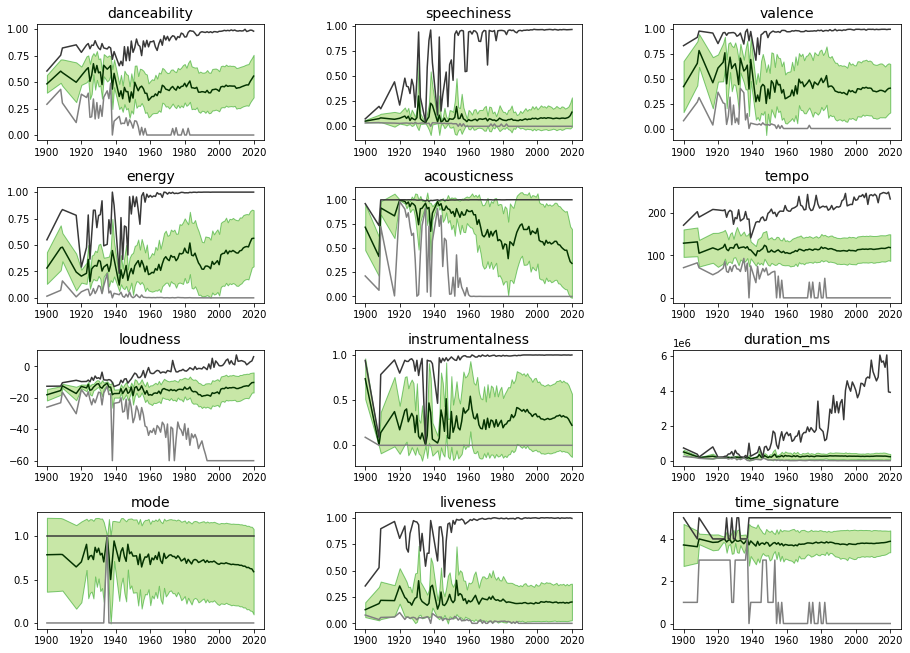
\includegraphics[width=\textwidth]{images/over_time.png}
\caption{Entwicklung der Musik-Attribute von 1900 bis 2020. Die in der Mitte verlaufende Linie ist der Durchschnittswert, die obere Linie das Maximum, die untere Linie das Minimum und der grüne Bereich ist die Standardabweichung im gegebenen Jahr.}
\label{time}
\end{figure*}
Aus den vorliegenden Daten geht hervor, dass sich die Musik im Laufe der Jahre in Bezug auf verschiedene Attribute deutlich verändert hat, und gewisse Trends ersichtlich sind. Die Analyse bezieht sich auf Abbildung \ref{time}. Im Folgenden werden nicht alle Attribute aufgegriffen, da bei ihnen Statistiken wie Standardabweichung und Durchschnittswert weniger aussagekräftig sind (bspw "Key" also der Notenschlüssel).

\begin{itemize}
\item{Danceability} Beginnend mit der danceability sehen wir, dass der Mindestwert und der Maximalwert über die Jahre leicht auseinander gehen. Nach einem Absinken der danceability in den 1940 Jahren zeigt der Durchschnittswert wieder einen leichten Aufwärtstrend. Die Standardabweichung bleibt relativ stabil über die Zeit.

\item{Eneregy} Auch bei der Energie ist ein ähnlicher Trend zu beobachten: Der Minimalwert bleibt relativ konstant, der Maximalwert steigt stetig an, der Durchschnittswert zeigt einen Aufwärtstrend und die Standardabweichung nimmt im Laufe der Zeit zu. Dies deutet darauf hin, dass die Musik im Laufe der Jahre energiegeladener geworden ist, es gleichzeitig aber mehr Diversität in diesem Attribut gibt.

\item{Loudness} Bei der Lautstärke ist ein sinkender Minimalwert und eine starke Zunahme des Maximalwerts zu verzeichnen, während der Durchschnitt relativ konstant bei ca. 4 Minuten und 6 Sekunden mit nur geringer Standardabweichung bleibt.

\item{Mode} Der Durchschnittswert des Modus bleibt über die gesamte Zeit überhalb von 0.5, was aussagt, dass stets mehr Musik in Dur produziert wird als in Moll, wobei ein leichter Abstieg des Durchschnittswertes in den letzten jahren zu verzeichnen ist. Es wurde also in den letzten Jahren mehr in Moll produziert. Die Standardabweichung bleibt konstant hoch der Modus nur zwei Werte annehmen kann.

\item{Speechiness} Das Minimum des Sprachanteils bleibt nahe bei 0, da Instrumentalmusik früher wie auch heute relevant ist. Der anfangs geringe Maximalwert entwickelt sich hingegen nach oben. Durchschnittswert und Standardabweichung bleiben gering was darauf hindeutet das der Großteil der Musik nach wie vor instrumental ist. Die Sprachlichkeit zeigt einen konstanten Rückgang der Minimal-, Maximal- und Durchschnittswerte, was darauf hindeutet, dass die Musik im Laufe der Jahre weniger sprachorientiert geworden ist. 

\item{Acousticness} Die Akustizität zeigt einen konstanten Rückgang der Durchschnittswerte, was darauf hindeutet, dass die Musik im Laufe der Jahre elektronischer geworden ist. Die Standardabweichung für das Attribut "Akustizität" nimmt im Laufe der Zeit zu, was darauf hindeutet, dass die Verteilung der Akustizitätswerte im Laufe der Zeit immer vielfältiger und unterschiedlicher wird. Elektronische Musik ersetzt akustische Musik also nicht, sondern kommt zusätzlich hinzu. Es könnte auch darauf hindeuten, dass die Definition oder Interpretation dessen, was als "akustische" Musik gilt, nuancierter und vielfältiger wird.

\item{instrumentalness} Bei der Instrumentalität ist ein auf und ab zu sehen, ohne klaren Trend hinsichtlich wachsendem oder fallendem Instrumentalanteil. Die Standardabweichung bleibt konsistent hoch, was bedeutet, dass nach wie vor viele Lieder mit hohem als auch niedrigem Instrumentalanteil produziert werden.

\item{liveness} Auch "Liveness" zeigt keinen eindeutigen Trend. Der Durchschnittswert ist relativ niedrig mit einer geringen Standardabweichung, was darauf hindeutet dass der Großteil der Musik nicht "live" aufgenommen wurde und immernoch wird.

\item{valence} Die Valenz zeigt keinen konstanten Abstieg der Statistiken, aber einen Reduktion des Durchschnittswerts ab den 1940ern ähnlich zur danceability, was darauf hindeutet, dass die Musik seit dieser Zeit weniger positiv ist.

\item{Tempo} Das Maximaltempo wird über die Jahre höher und das Minimaltempo wird niedriger während der Durchschnittswert relativ konstant im mittleren Bereich der Attributskala bleibt. Die Standardabweichung ist niedrig und konstant. Die meisten Lieder sind also weder langsam noch schnell, aber es wird über die Jahre immer wieder mit neuen Tempo-Rekorden experimentiert.

\item{Duration} (Dauer): Die Dauer zeigt einen starken Anstieg des Maximalwertes. Minimal- und Durchschnittswerte bleiben relativ konsistent und gering, genauso wie die Standardabweichung, das heißt die Musik ist in Bezug auf die Dauer stabil.

\item{Time signature} Der Anteil der Songs mit 4/4-Takt ist im Laufe der Zeit relativ stabil geblieben, die meisten Songs sind im 4/4-Takt, die Standardabweichung der Taktart ist gering und im Laufe der Zeit stabil, was darauf hindeutet, dass die meisten Songs hauptsächlich im 4/4-Takt sind.
\end{itemize}

Insgesamt hat es den Anschein, dass die Musik im Laufe der Jahre energiegeladener und etwas tanzbarer und lauter geworden ist, wobei die durchschnittliche Tanzbarkeit und das Energieniveau allmählich gestiegen sind. Die durchschnittliche Akustik und Instrumentalität schwanken. Die Musik scheint aber insgesamt zu mehr elektronischen oder synthetischen Klängen zu tendieren, da sich der Anteil der akustischen Musik über die Jahre eindeutig verringert. Für die Attribute deren Durchschnittswert einem klaren Trend folgt, also der relative Rückgang akustischer Elemente und der Anstieg der Energie, lässt sich auch ein Anstieg in der Standardabweichung, also der Diversität in der Ausprägung des Attributs feststellen.

\section{Ease of Use}

\subsection{Maintaining the Integrity of the Specifications}

The IEEEtran class file is used to format your paper and style the text. All margins, 
column widths, line spaces, and text fonts are prescribed; please do not 
alter them. You may note peculiarities. For example, the head margin
measures proportionately more than is customary. This measurement 
and others are deliberate, using specifications that anticipate your paper 
as one part of the entire proceedings, and not as an independent document. 
Please do not revise any of the current designations.

\section{Prepare Your Paper Before Styling}
Before you begin to format your paper, first write and save the content as a 
separate text file. Complete all content and organizational editing before 
formatting. Please note sections \ref{AA}--\ref{SCM} below for more information on 
proofreading, spelling and grammar.

Keep your text and graphic files separate until after the text has been 
formatted and styled. Do not number text heads---{\LaTeX} will do that 
for you.

\subsection{Abbreviations and Acronyms}\label{AA}
Define abbreviations and acronyms the first time they are used in the text, 
even after they have been defined in the abstract. Abbreviations such as 
IEEE, SI, MKS, CGS, ac, dc, and rms do not have to be defined. Do not use 
abbreviations in the title or heads unless they are unavoidable.

\subsection{Units}
\begin{itemize}
\item Use either SI (MKS) or CGS as primary units. (SI units are encouraged.) English units may be used as secondary units (in parentheses). An exception would be the use of English units as identifiers in trade, such as ``3.5-inch disk drive''.
\item Avoid combining SI and CGS units, such as current in amperes and magnetic field in oersteds. This often leads to confusion because equations do not balance dimensionally. If you must use mixed units, clearly state the units for each quantity that you use in an equation.
\item Do not mix complete spellings and abbreviations of units: ``Wb/m\textsuperscript{2}'' or ``webers per square meter'', not ``webers/m\textsuperscript{2}''. Spell out units when they appear in text: ``. . . a few henries'', not ``. . . a few H''.
\item Use a zero before decimal points: ``0.25'', not ``.25''. Use ``cm\textsuperscript{3}'', not ``cc''.)
\end{itemize}

\subsection{Equations}
Number equations consecutively. To make your 
equations more compact, you may use the solidus (~/~), the exp function, or 
appropriate exponents. Italicize Roman symbols for quantities and variables, 
but not Greek symbols. Use a long dash rather than a hyphen for a minus 
sign. Punctuate equations with commas or periods when they are part of a 
sentence, as in:
\begin{equation}
a+b=\gamma\label{eq}
\end{equation}

Be sure that the 
symbols in your equation have been defined before or immediately following 
the equation. Use ``\eqref{eq}'', not ``Eq.~\eqref{eq}'' or ``equation \eqref{eq}'', except at 
the beginning of a sentence: ``Equation \eqref{eq} is . . .''

\subsection{\LaTeX-Specific Advice}

Please use ``soft'' (e.g., \verb|\eqref{Eq}|) cross references instead
of ``hard'' references (e.g., \verb|(1)|). That will make it possible
to combine sections, add equations, or change the order of figures or
citations without having to go through the file line by line.

Please don't use the \verb|{eqnarray}| equation environment. Use
\verb|{align}| or \verb|{IEEEeqnarray}| instead. The \verb|{eqnarray}|
environment leaves unsightly spaces around relation symbols.

Please note that the \verb|{subequations}| environment in {\LaTeX}
will increment the main equation counter even when there are no
equation numbers displayed. If you forget that, you might write an
article in which the equation numbers skip from (17) to (20), causing
the copy editors to wonder if you've discovered a new method of
counting.

{\BibTeX} does not work by magic. It doesn't get the bibliographic
data from thin air but from .bib files. If you use {\BibTeX} to produce a
bibliography you must send the .bib files. 

{\LaTeX} can't read your mind. If you assign the same label to a
subsubsection and a table, you might find that Table I has been cross
referenced as Table IV-B3. 

{\LaTeX} does not have precognitive abilities. If you put a
\verb|\label| command before the command that updates the counter it's
supposed to be using, the label will pick up the last counter to be
cross referenced instead. In particular, a \verb|\label| command
should not go before the caption of a figure or a table.

Do not use \verb|\nonumber| inside the \verb|{array}| environment. It
will not stop equation numbers inside \verb|{array}| (there won't be
any anyway) and it might stop a wanted equation number in the
surrounding equation.

\subsection{Some Common Mistakes}\label{SCM}
\begin{itemize}
\item The word ``data'' is plural, not singular.
\item The subscript for the permeability of vacuum $\mu_{0}$, and other common scientific constants, is zero with subscript formatting, not a lowercase letter ``o''.
\item In American English, commas, semicolons, periods, question and exclamation marks are located within quotation marks only when a complete thought or name is cited, such as a title or full quotation. When quotation marks are used, instead of a bold or italic typeface, to highlight a word or phrase, punctuation should appear outside of the quotation marks. A parenthetical phrase or statement at the end of a sentence is punctuated outside of the closing parenthesis (like this). (A parenthetical sentence is punctuated within the parentheses.)
\item A graph within a graph is an ``inset'', not an ``insert''. The word alternatively is preferred to the word ``alternately'' (unless you really mean something that alternates).
\item Do not use the word ``essentially'' to mean ``approximately'' or ``effectively''.
\item In your paper title, if the words ``that uses'' can accurately replace the word ``using'', capitalize the ``u''; if not, keep using lower-cased.
\item Be aware of the different meanings of the homophones ``affect'' and ``effect'', ``complement'' and ``compliment'', ``discreet'' and ``discrete'', ``principal'' and ``principle''.
\item Do not confuse ``imply'' and ``infer''.
\item The prefix ``non'' is not a word; it should be joined to the word it modifies, usually without a hyphen.
\item There is no period after the ``et'' in the Latin abbreviation ``et al.''.
\item The abbreviation ``i.e.'' means ``that is'', and the abbreviation ``e.g.'' means ``for example''.
\end{itemize}
An excellent style manual for science writers is \cite{b7}.

\subsection{Authors and Affiliations}
\textbf{The class file is designed for, but not limited to, six authors.} A 
minimum of one author is required for all conference articles. Author names 
should be listed starting from left to right and then moving down to the 
next line. This is the author sequence that will be used in future citations 
and by indexing services. Names should not be listed in columns nor group by 
affiliation. Please keep your affiliations as succinct as possible (for 
example, do not differentiate among departments of the same organization).

\subsection{Identify the Headings}
Headings, or heads, are organizational devices that guide the reader through 
your paper. There are two types: component heads and text heads.

Component heads identify the different components of your paper and are not 
topically subordinate to each other. Examples include Acknowledgments and 
References and, for these, the correct style to use is ``Heading 5''. Use 
``figure caption'' for your Figure captions, and ``table head'' for your 
table title. Run-in heads, such as ``Abstract'', will require you to apply a 
style (in this case, italic) in addition to the style provided by the drop 
down menu to differentiate the head from the text.

Text heads organize the topics on a relational, hierarchical basis. For 
example, the paper title is the primary text head because all subsequent 
material relates and elaborates on this one topic. If there are two or more 
sub-topics, the next level head (uppercase Roman numerals) should be used 
and, conversely, if there are not at least two sub-topics, then no subheads 
should be introduced.

\subsection{Figures and Tables}
\paragraph{Positioning Figures and Tables} Place figures and tables at the top and 
bottom of columns. Avoid placing them in the middle of columns. Large 
figures and tables may span across both columns. Figure captions should be 
below the figures; table heads should appear above the tables. Insert 
figures and tables after they are cited in the text. Use the abbreviation 
``Fig.~\ref{fig}'', even at the beginning of a sentence.

\begin{table}[htbp]
\caption{Table Type Styles}
\begin{center}
\begin{tabular}{|c|c|c|c|}
\hline
\textbf{Table}&\multicolumn{3}{|c|}{\textbf{Table Column Head}} \\
\cline{2-4} 
\textbf{Head} & \textbf{\textit{Table column subhead}}& \textbf{\textit{Subhead}}& \textbf{\textit{Subhead}} \\
\hline
copy& More table copy$^{\mathrm{a}}$& &  \\
\hline
\multicolumn{4}{l}{$^{\mathrm{a}}$Sample of a Table footnote.}
\end{tabular}
\label{tab1}
\end{center}
\end{table}

\begin{figure}[htbp]
\centerline{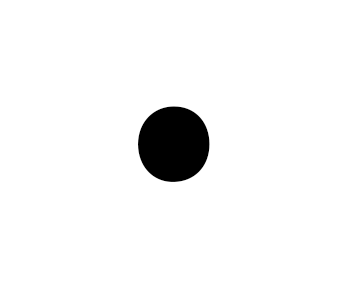
\includegraphics{fig1.png}}
\caption{Example of a figure caption.}
\label{fig}
\end{figure}

Figure Labels: Use 8 point Times New Roman for Figure labels. Use words 
rather than symbols or abbreviations when writing Figure axis labels to 
avoid confusing the reader. As an example, write the quantity 
``Magnetization'', or ``Magnetization, M'', not just ``M''. If including 
units in the label, present them within parentheses. Do not label axes only 
with units. In the example, write ``Magnetization (A/m)'' or ``Magnetization 
\{A[m(1)]\}'', not just ``A/m''. Do not label axes with a ratio of 
quantities and units. For example, write ``Temperature (K)'', not 
``Temperature/K''.

\section*{Acknowledgment}

The preferred spelling of the word ``acknowledgment'' in America is without 
an ``e'' after the ``g''. Avoid the stilted expression ``one of us (R. B. 
G.) thanks $\ldots$''. Instead, try ``R. B. G. thanks$\ldots$''. Put sponsor 
acknowledgments in the unnumbered footnote on the first page.

\section*{References}

Please number citations consecutively within brackets \cite{b1}. The 
sentence punctuation follows the bracket \cite{b2}. Refer simply to the reference 
number, as in \cite{b3}---do not use ``Ref. \cite{b3}'' or ``reference \cite{b3}'' except at 
the beginning of a sentence: ``Reference \cite{b3} was the first $\ldots$''

Number footnotes separately in superscripts. Place the actual footnote at 
the bottom of the column in which it was cited. Do not put footnotes in the 
abstract or reference list. Use letters for table footnotes.

Unless there are six authors or more give all authors' names; do not use 
``et al.''. Papers that have not been published, even if they have been 
submitted for publication, should be cited as ``unpublished'' \cite{b4}. Papers 
that have been accepted for publication should be cited as ``in press'' \cite{b5}. 
Capitalize only the first word in a paper title, except for proper nouns and 
element symbols.

For papers published in translation journals, please give the English 
citation first, followed by the original foreign-language citation \cite{b6}.

\begin{thebibliography}{00}
\bibitem{d1} Pichl, Martin; Zangerle, Eva; Specht, Günther: "Towards a Context-Aware Music Recommendation Approach: What is Hidden in the Playlist Name?" in 15th IEEE International Conference on Data Mining Workshops (ICDM 2015), pp. 1360-1365, IEEE, Atlantic City, 2015.
\bibitem{d2} Figueroa, Rodolfo. (2020). Spotify 12M Songs [Dataset]. Kaggle. https://www.kaggle.com/datasets/rodolfofigueroa/spotify-12m-songs

\bibitem{b1} G. Eason, B. Noble, and I. N. Sneddon, ``On certain integrals of Lipschitz-Hankel type involving products of Bessel functions,'' Phil. Trans. Roy. Soc. London, vol. A247, pp. 529--551, April 1955.
\bibitem{b2} J. Clerk Maxwell, A Treatise on Electricity and Magnetism, 3rd ed., vol. 2. Oxford: Clarendon, 1892, pp.68--73.
\bibitem{b3} I. S. Jacobs and C. P. Bean, ``Fine particles, thin films and exchange anisotropy,'' in Magnetism, vol. III, G. T. Rado and H. Suhl, Eds. New York: Academic, 1963, pp. 271--350.
\bibitem{b4} K. Elissa, ``Title of paper if known,'' unpublished.
\bibitem{b5} R. Nicole, ``Title of paper with only first word capitalized,'' J. Name Stand. Abbrev., in press.
\bibitem{b6} Y. Yorozu, M. Hirano, K. Oka, and Y. Tagawa, ``Electron spectroscopy studies on magneto-optical media and plastic substrate interface,'' IEEE Transl. J. Magn. Japan, vol. 2, pp. 740--741, August 1987 [Digests 9th Annual Conf. Magnetics Japan, p. 301, 1982].
\bibitem{b7} M. Young, The Technical Writer's Handbook. Mill Valley, CA: University Science, 1989.
\end{thebibliography}
\vspace{12pt}
\color{red}
IEEE conference templates contain guidance text for composing and formatting conference papers. Please ensure that all template text is removed from your conference paper prior to submission to the conference. Failure to remove the template text from your paper may result in your paper not being published.

\end{document}
